\documentclass{standalone}

\usepackage{tikz}
\usetikzlibrary{shapes.geometric}
\begin{document}
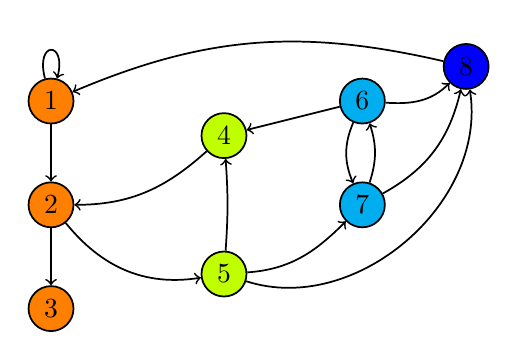
\begin{tikzpicture}
[every node/.style={inner sep=0pt}]
\node (4) [circle, minimum size=16.25pt, fill=lime, line width=0.625pt, draw=black] at (125.0pt, -37.5pt) {\textcolor{black}{4}};
\node (5) [circle, minimum size=16.25pt, fill=lime, line width=0.625pt, draw=black] at (125.0pt, -87.5pt) {\textcolor{black}{5}};
\node (1) [circle, minimum size=16.25pt, fill=orange, line width=0.625pt, draw=black] at (62.5pt, -25.0pt) {\textcolor{black}{1}};
\node (2) [circle, minimum size=16.25pt, fill=orange, line width=0.625pt, draw=black] at (62.5pt, -62.5pt) {\textcolor{black}{2}};
\node (3) [circle, minimum size=16.25pt, fill=orange, line width=0.625pt, draw=black] at (62.5pt, -100.0pt) {\textcolor{black}{3}};
\node (8) [circle, minimum size=16.25pt, fill=blue, line width=0.625pt, draw=black] at (212.5pt, -12.5pt) {\textcolor{black}{8}};
\node (6) [circle, minimum size=16.25pt, fill=cyan, line width=0.625pt, draw=black] at (175.0pt, -25.0pt) {\textcolor{black}{6}};
\node (7) [circle, minimum size=16.25pt, fill=cyan, line width=0.625pt, draw=black] at (175.0pt, -62.5pt) {\textcolor{black}{7}};
\draw [line width=0.625, ->, color=black, loop above] (1) to (1);
\draw [line width=0.625, ->, color=black] (1) to  (2);
\draw [line width=0.625, ->, color=black] (2) to  (3);
\draw [line width=0.625, ->, color=black] (5) to  [in=274, out=86] (4);
\draw [line width=0.625, ->, color=black] (4) to  [in=0, out=222] (2);
\draw [line width=0.625, ->, color=black] (7) to  [in=257, out=29] (8);
\draw [line width=0.625, ->, color=black] (8) to  [in=23, out=167] (1);
\draw [line width=0.625, ->, color=black] (2) to  [in=189, out=309] (5);
\draw [line width=0.625, ->, color=black] (5) to  [in=225, out=4] (7);
\draw [line width=0.625, ->, color=black] (6) to  (4);
\draw [line width=0.625, ->, color=black] (7) to  [in=288, out=72] (6);
\draw [line width=0.625, ->, color=black] (6) to  [in=113, out=247] (7);
\draw [line width=0.625, ->, color=black] (6) to  [in=225, out=356] (8);
\draw [line width=0.625, ->, color=black] (5) to  [in=279, out=342] (8);
\end{tikzpicture}
\end{document}
